
\section{Data Plane Properties}
In this section, we discuss three different data plane properties and mechanisms to support them atop the control logic.

\subsection{Loss-Free Update}

%In the migration control logic, we have the concept of ``path''; let us now only focus on data plane and see how path is reflected there.

At the data plane, there is a translation table stored in each middlebox. The \system agent accepts flows for which it has established state, rewrites the header, and forwards the flow based on the supersession-subsession mapping. Moving a flow from one path to another is equivalent to updating the translation tables at the data plane to accept a flow from the new subsession(s) and reject the same flow from the old subsessions. Since there are multiple middleboxes involved in the update procedure, the update order matters. Otherwise, the translation layer may drop packets if the update happens in the wrong order, for example if the old subsession is removed before the new subsession is fully established.


Finding the right sequence of updates for a general network is proven to be NP-complete~\cite{SWAN, zUpdate}, but for a special topology, linear in our setting (we only abstract the topology between middleboxes), we can apply the concept from network consistent update~\cite{consistentupdate, ratul}. We first ensure that the new translation rules are all pushed before the egress applies the new rule, and the old rules are not removed until all the new rules are installed via a complete handshake. In particular, when a migration is initialized from the middlebox (a signaling point), the middlebox notifies its neighbor through the control plane, which inserts a new rule for incoming traffic. Then this neighbor notifies the other side of the connection with an UPDATE-SYN control message. Every hop that receives UPDATE-SYN updates its own translation table. Hence once the other signaling endpoint receives the notification, a new rule for the flow has been installed at every hop for one direction of traffic; it is thus safe to apply the new rule for the egress. The opposite direction is set up via the same way with UPDATE-SYNACK messages. Once the new bidirectional path is built, we tear down the old path by removing the old rules. This loss-free update mechanism mirrors the control plane ``make before break'' philosophy and is in fact facilitated by the control plane design. 

 \begin{figure}[ht]
\centering
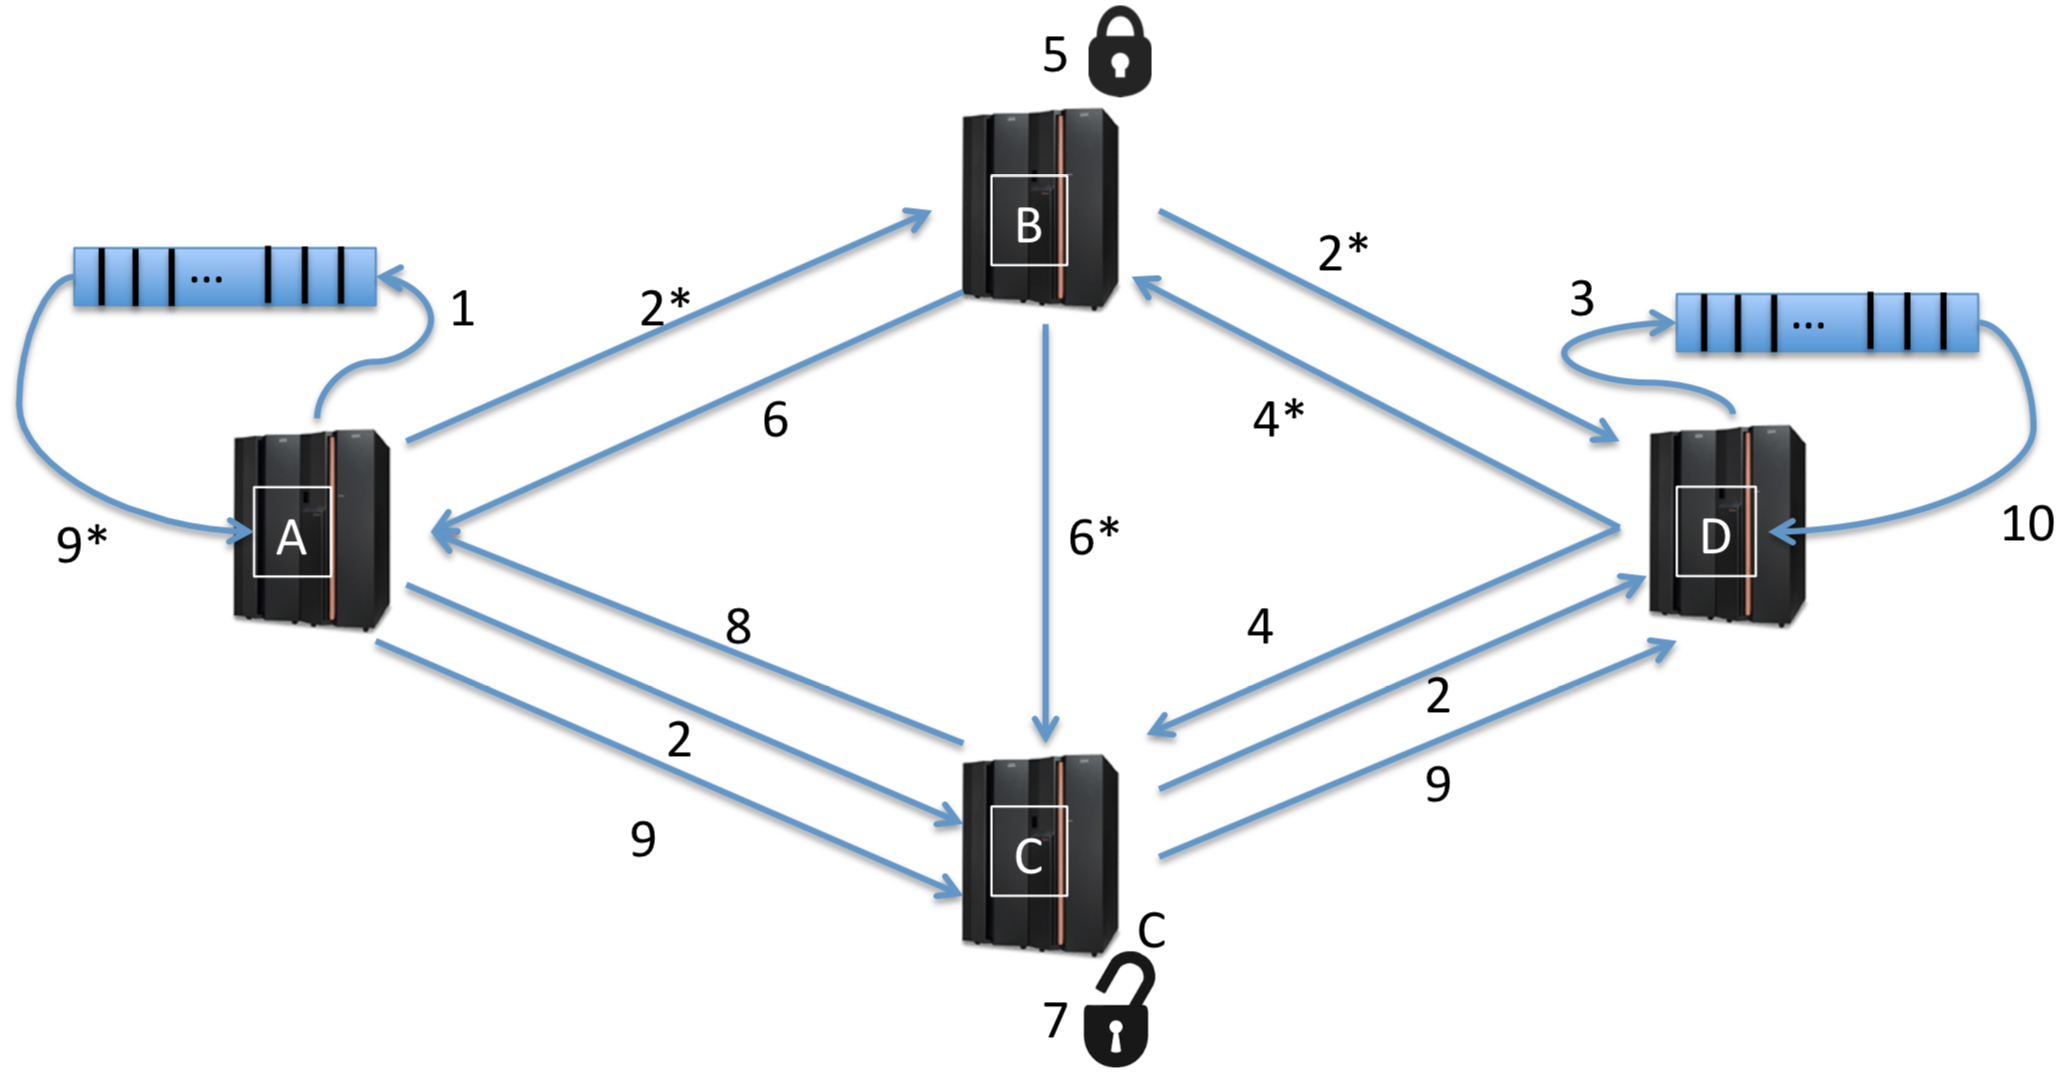
\includegraphics[width=\linewidth]{figures/order_preserving.png} 

\caption{Flow Migration} \label{orderpreserving} 
\end{figure}
 
\subsection{Packet Order Preserving} \label{FIFO}
The previously described loss-free update is insufficient if the NF instance (state) also needs to migrate. More specifically, the NF state cannot be migrated since it is being continuously updated as packets are coming in via the old path. To lock and migrate the middlebox state, \system must stop sending traffic during the new path setup. Since changing the protocols' (e.g., TCP) flow control is undesirable, we choose to buffer the traffic and not to release it until the network function state on the old path's middlebox has been locked and replicated to the new path's middlebox. Since NF state replication and migration is a well solved problem~\cite{OpenNF, splitmerge, HAMbox}, we do not address this problem here. 

The migration takes 10 steps\footnote{$x$ and $x*$ can happen in parallel where $x$ is a number.} as depicted in Figure~\ref{orderpreserving}: 
1. lock outgoing traffic; 
2. send UPDATE-SYN via new path; 
2*. send UPDATE-FIN via old path;
3. lock the reverse direction traffic;
4. send UPDATE-SYNACK via new path;
4*. send UPDATE-FINACK via old path;
5. lock middlebox states;
6. send UPDATE-FINACK via old path;
6*. migrate states;
7. unlock middlebox states;
8. send UPDATE-SYNACK via new path;
9*. release buffered traffic;
9. send ACK packets;
10. release buffered traffic for the other direction.
\newline


\begin{figure}[ht]
\centering
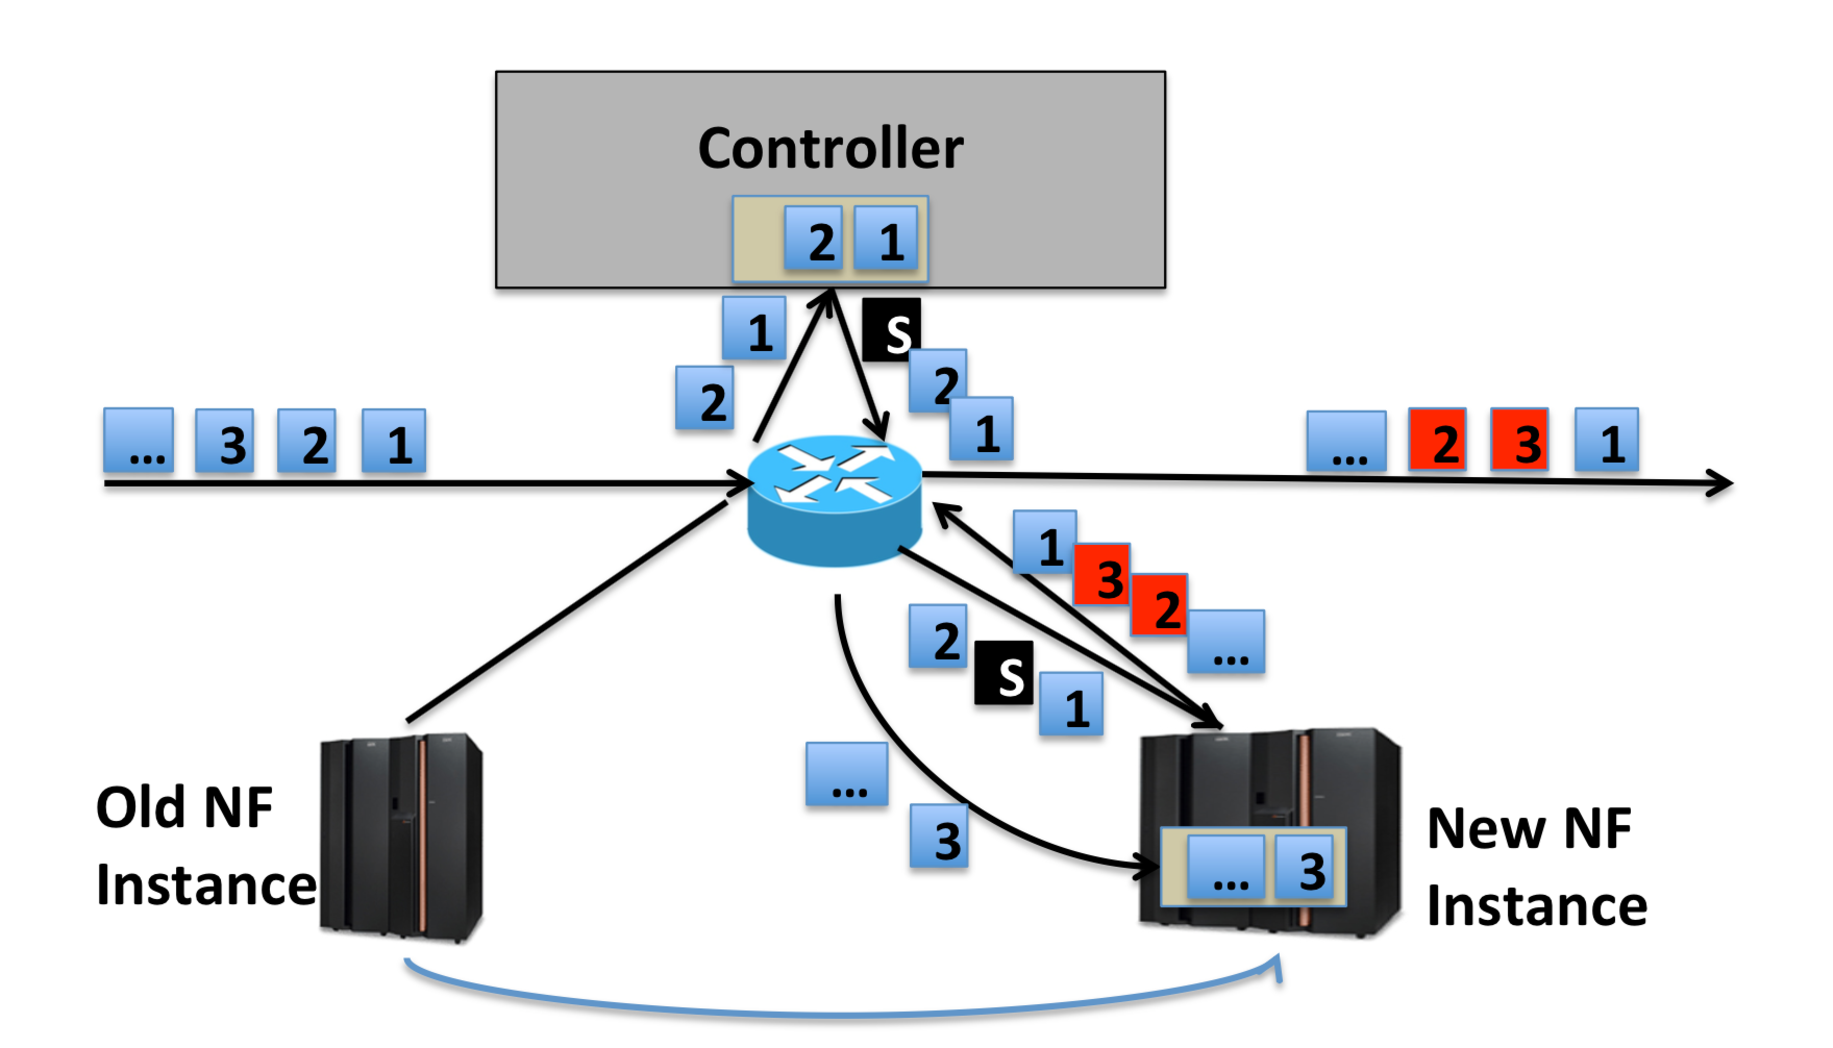
\includegraphics[width=\linewidth]{figures/opennfbroke.pdf} 
\caption{\small Order-preserving problem in OpenNF without FIFO assumption, the signal packet s and the data packets 1 and 2 maybe reordered and thus create reordering. Note the switch is one big switch abstraction.}\label{opennfbroke}
\end{figure}


The update mechanism above is also order-preserving under the same assumption in OpenNF: the path to NF instance is \textbf{FIFO}, i.e., the notification message sent after the last data packet is always received after the last data packet, whereas the \textbf{Order-Preserving} property is defined as the following: \textit{All packets should be processed in the order they were forwarded to the NF instance by the switch (network)}~\cite{OpenNF}. 
 
\subsection{Substream Separation and Order Preserving}  
Creating a separation of two substreams for a byte stream (e.g., TCP) is beneficial to avoid false alert from NFs and/or improve the NF efficiency. When we plan to migrate a flow from one IDS to another, we may want to ensure that all the SYNs and corresponding ACKs are going through the same IDS, otherwise, it may raise an alert like ``ACK before SYN''. When the flow passes through a deep packet inspection (DPI), both string matching and reg-exp matching builds a Deterministic Finite Automaton (DFA) first, and traverses from the root to certain state based on the byte stream~\cite{aho, yaron}. If we want to use different DPI instances for a byte stream, and the first instance has not seen a complete substream, it can only check the largest continuous byte stream, buffer the remaining bytes and send to the second instance.  

 
To lock the traffic and separate the substream, the left neighbor of the moving point use the maximum seen sequence number as a \textit{checkpoint}, and buffers the packets with a higher sequence number than the checkpoint and forwards the packets with a lower sequence number. We do not lock and migrate the old NF instance state until seeing an ACK at sequence number \textit{checkpoint}. This guarantees the delivery of the packets at the old path since ACK is sent from an endpoint. Note this may create a reordering from the perspective of the left neighbor middlebox, however this is not a reordering from the perspective of endpoints. See Algorithm~\ref{strictorderpres} for details. 

We may need to split the packets in the case of \textit{SYN-ACK piggyback and packet coalescing}: In the first case, if both directions ask for substream separation, we may get in a deadlock since \system may choose the new path for a substream with higher sequence number in one direction and the old path for ACK as it is acking a substream with lower sequence number in the reversed direction; in the second case, TCP client may coalesce packets and the payload  may cross the \textit{checkpoint} boundary in the byte stream if retransmission occurs. 

\begin{algorithm} [htbp]
\footnotesize
\SetAlgoLined
\SetKwFunction{syn}{recv\_SYN}\SetKwFunction{ack}{recv\_ACK}\SetKwFunction{queue}{release\_queue}
\SetKwProg{mypacket}{Event\_Handler}{}{}
\SetKwProg{func}{Program}{}{}

\mypacket{\syn{TCP\_packet p} } {
checkpoint = hash\_lookup(p)\;
\If{p.seq $>$ checkpoint} {
Buffer (p)\;
} 
\Else{Forward(p)\;}
} 




\mypacket{\ack{TCP\_packet p}}{
\If{p.ack $>$checkpoint}{
Migrate NF state\;
//wait until migration finishes\;
sendto(left neighbor, release\_buffer)\;
}
}


\mypacket{\queue{}}{
\While{!buffer.empty()}{
Forward(buffer.dequeue())\;
}
Reset(hash\_table)\;
}

\caption{Substream Separation and Order Preserving} \label{strictorderpres}


\end{algorithm} 


A combination of order preserving and substream separation provides us with a stronger order preserving during an update: \textit{Packets should be processed by different NF instances in the order they were sent from the sender}. OpenNF cannot guarantee order preserving, when certain network links are not FIFO~\footnote{OpenNF tech report relies on this assumption in its proof.}, nor can OpenNF be extended due to its design choice (i.e., routing based), as shown in Figure~\ref{opennfbroke} . Our protocol is able to provide this property precisely because the system architecture is designed to be aware of and rely on transport protocols.



